% Options for packages loaded elsewhere
\PassOptionsToPackage{unicode}{hyperref}
\PassOptionsToPackage{hyphens}{url}
\PassOptionsToPackage{dvipsnames,svgnames,x11names}{xcolor}
%
\documentclass[
  12pt,
]{article}
\usepackage{amsmath,amssymb}
\usepackage{iftex}
\ifPDFTeX
  \usepackage[T1]{fontenc}
  \usepackage[utf8]{inputenc}
  \usepackage{textcomp} % provide euro and other symbols
\else % if luatex or xetex
  \usepackage{unicode-math} % this also loads fontspec
  \defaultfontfeatures{Scale=MatchLowercase}
  \defaultfontfeatures[\rmfamily]{Ligatures=TeX,Scale=1}
\fi
\usepackage{lmodern}
\ifPDFTeX\else
  % xetex/luatex font selection
\fi
% Use upquote if available, for straight quotes in verbatim environments
\IfFileExists{upquote.sty}{\usepackage{upquote}}{}
\IfFileExists{microtype.sty}{% use microtype if available
  \usepackage[]{microtype}
  \UseMicrotypeSet[protrusion]{basicmath} % disable protrusion for tt fonts
}{}
\makeatletter
\@ifundefined{KOMAClassName}{% if non-KOMA class
  \IfFileExists{parskip.sty}{%
    \usepackage{parskip}
  }{% else
    \setlength{\parindent}{0pt}
    \setlength{\parskip}{6pt plus 2pt minus 1pt}}
}{% if KOMA class
  \KOMAoptions{parskip=half}}
\makeatother
\usepackage{xcolor}
\usepackage[margin=1in]{geometry}
\usepackage{longtable,booktabs,array}
\usepackage{calc} % for calculating minipage widths
% Correct order of tables after \paragraph or \subparagraph
\usepackage{etoolbox}
\makeatletter
\patchcmd\longtable{\par}{\if@noskipsec\mbox{}\fi\par}{}{}
\makeatother
% Allow footnotes in longtable head/foot
\IfFileExists{footnotehyper.sty}{\usepackage{footnotehyper}}{\usepackage{footnote}}
\makesavenoteenv{longtable}
\usepackage{graphicx}
\makeatletter
\def\maxwidth{\ifdim\Gin@nat@width>\linewidth\linewidth\else\Gin@nat@width\fi}
\def\maxheight{\ifdim\Gin@nat@height>\textheight\textheight\else\Gin@nat@height\fi}
\makeatother
% Scale images if necessary, so that they will not overflow the page
% margins by default, and it is still possible to overwrite the defaults
% using explicit options in \includegraphics[width, height, ...]{}
\setkeys{Gin}{width=\maxwidth,height=\maxheight,keepaspectratio}
% Set default figure placement to htbp
\makeatletter
\def\fps@figure{htbp}
\makeatother
\setlength{\emergencystretch}{3em} % prevent overfull lines
\providecommand{\tightlist}{%
  \setlength{\itemsep}{0pt}\setlength{\parskip}{0pt}}
\setcounter{secnumdepth}{5}
\newlength{\cslhangindent}
\setlength{\cslhangindent}{1.5em}
\newlength{\csllabelwidth}
\setlength{\csllabelwidth}{3em}
\newlength{\cslentryspacingunit} % times entry-spacing
\setlength{\cslentryspacingunit}{\parskip}
\newenvironment{CSLReferences}[2] % #1 hanging-ident, #2 entry spacing
 {% don't indent paragraphs
  \setlength{\parindent}{0pt}
  % turn on hanging indent if param 1 is 1
  \ifodd #1
  \let\oldpar\par
  \def\par{\hangindent=\cslhangindent\oldpar}
  \fi
  % set entry spacing
  \setlength{\parskip}{#2\cslentryspacingunit}
 }%
 {}
\usepackage{calc}
\newcommand{\CSLBlock}[1]{#1\hfill\break}
\newcommand{\CSLLeftMargin}[1]{\parbox[t]{\csllabelwidth}{#1}}
\newcommand{\CSLRightInline}[1]{\parbox[t]{\linewidth - \csllabelwidth}{#1}\break}
\newcommand{\CSLIndent}[1]{\hspace{\cslhangindent}#1}
\usepackage{setspace} \usepackage{amssymb} \usepackage{amsmath} \setstretch{1.15} \usepackage{float} \floatplacement{figure}{t}
\ifLuaTeX
  \usepackage{selnolig}  % disable illegal ligatures
\fi
\IfFileExists{bookmark.sty}{\usepackage{bookmark}}{\usepackage{hyperref}}
\IfFileExists{xurl.sty}{\usepackage{xurl}}{} % add URL line breaks if available
\urlstyle{same}
\hypersetup{
  colorlinks=true,
  linkcolor={cyan},
  filecolor={Maroon},
  citecolor={Blue},
  urlcolor={cyan},
  pdfcreator={LaTeX via pandoc}}

\title{~\Large Indian Premier League Cricket}
\author{\large Matthew Stuart\(^{1,2}\), Hassan Raffique\(^{3}\), Leigha
DeRango\(^1\)\\
\large Gregory J. Matthews\(^{1,2}\)\\
\vspace{-1.1mm}\\
\large \(^1\) Department of Mathematics and Statistics, Loyola
University Chicago, Chicago, IL, USA \vspace{-1.1mm}\\
\large \(^2\) Center for Data Science and Consulting, Loyola University
Chicago, Chicago, IL, USA \vspace{-1.1mm}\\
\large \(^3\) University of Iowa, Iowa City, IA \vspace{-1.1mm}\\
\large \(^+\) Corresponding:
\href{mailto:mstuart1@luc.edu}{\nolinkurl{mstuart1@luc.edu}}
\vspace{-1.1mm}}
\date{}

\begin{document}
\maketitle
\begin{abstract}
Wicked Googly \vspace{2mm}\\
\emph{Keywords}: Cricket
\end{abstract}

\newcommand{\iid}{\overset{iid}{\sim}}

\newpage

\hypertarget{sec:intro}{%
\section{Introduction}\label{sec:intro}}

openWAR and cricWAR.

In the game of cricket, the number of runs scored on a particular pitch
typically ranges between 0 and 6 (though theoretically values larger
than 6 are possible, they are rare and do not occur at all in our
particular data set).

\hypertarget{sec:data}{%
\section{Data}\label{sec:data}}

\begin{longtable}[]{@{}rr@{}}
\toprule\noalign{}
season & n\_teams \\
\midrule\noalign{}
\endhead
\bottomrule\noalign{}
\endlastfoot
2015 & 8 \\
2016 & 8 \\
2017 & 8 \\
2018 & 8 \\
2019 & 8 \\
2021 & 8 \\
2022 & 10 \\
\end{longtable}

We have data from the Indian Premier Leauge (IPL) consisting of 102490
pitches from the 2015 - 2022 seasons. From 2015 - 2021, the league had 8
teams followed by 10 teams in the 2022 season.

\begin{longtable}[]{@{}rr@{}}
\toprule\noalign{}
season & n\_pitches \\
\midrule\noalign{}
\endhead
\bottomrule\noalign{}
\endlastfoot
2015 & 13641 \\
2016 & 14096 \\
2017 & 13849 \\
2018 & 14286 \\
2019 & 14293 \\
2021 & 14413 \\
2022 & 17912 \\
\end{longtable}

Runs in cricket are either scored by running back and forth between the
wickets once the ball is put into play (generally resulting in 1 or 2
runs, but theoretically any value is possible). In addition, a ball that
is hit in the air over the boundary (termed a ``boundary'') is worth 6
runs and if the ball rolls to the boundary or bounces in the field of
play and then clears the boundary this is worth 4 runs (termed a
``boundary 4''). As a result the distribution of runs scored on a a
particular pitch has large peaks are 0 and 1 with a big drop off from 1
to 2. Values of 3 and 5 are extremely rare accounting for only 0.27\%
and 0.02\% of values across all pitches in our data set. Values of 4 and
6 spike because of boundaries and boundary fours and together account
for 16.75\% of all values.

\begin{figure}

{\centering 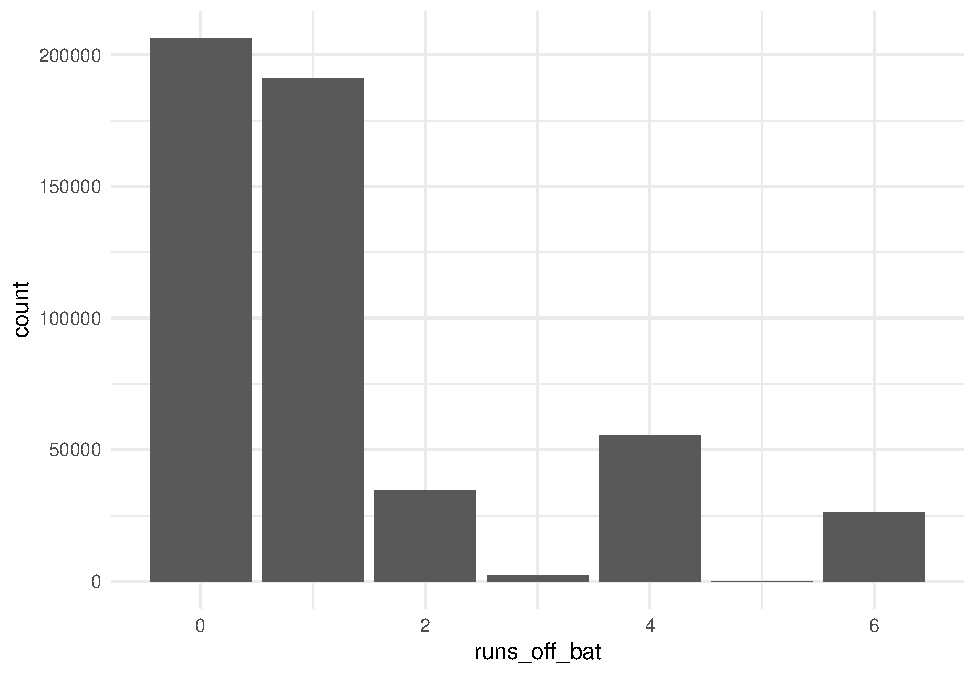
\includegraphics{paper_files/figure-latex/bar-1} 

}

\caption{Bar Plot of the number of runs scored of a particular ball}\label{fig:bar}
\end{figure}

\begin{longtable}[]{@{}lrr@{}}
\toprule\noalign{}
striker & xbar & n \\
\midrule\noalign{}
\endhead
\bottomrule\noalign{}
\endlastfoot
AD Russell & 1.725162 & 1077 \\
SP Narine & 1.633270 & 529 \\
AB de Villiers & 1.580799 & 1677 \\
RR Pant & 1.491333 & 1673 \\
GJ Maxwell & 1.459386 & 1108 \\
JC Buttler & 1.455233 & 1720 \\
JM Bairstow & 1.453149 & 651 \\
PP Shaw & 1.452991 & 936 \\
MM Ali & 1.411950 & 636 \\
DA Warner & 1.407686 & 2394 \\
BB McCullum & 1.404546 & 880 \\
RA Tripathi & 1.392540 & 1126 \\
CA Lynn & 1.387061 & 912 \\
KD Karthik & 1.382182 & 1549 \\
KL Rahul & 1.366216 & 2220 \\
KA Pollard & 1.360360 & 1332 \\
HH Pandya & 1.359741 & 1237 \\
CH Gayle & 1.358868 & 1449 \\
KH Pandya & 1.335895 & 911 \\
AJ Finch & 1.331909 & 702 \\
SV Samson & 1.328237 & 1962 \\
SA Yadav & 1.328021 & 1506 \\
DR Smith & 1.326897 & 725 \\
SR Watson & 1.321398 & 1173 \\
V Kohli & 1.317146 & 2677 \\
Q de Kock & 1.316218 & 1597 \\
RV Uthappa & 1.310302 & 1621 \\
PA Patel & 1.299277 & 1106 \\
RD Gaikwad & 1.299223 & 772 \\
N Rana & 1.290755 & 1417 \\
RG Sharma & 1.276062 & 2072 \\
MP Stoinis & 1.275311 & 563 \\
MA Agarwal & 1.268727 & 1068 \\
YK Pathan & 1.268182 & 880 \\
DJ Hooda & 1.266741 & 896 \\
MC Henriques & 1.263415 & 615 \\
AT Rayudu & 1.261749 & 1681 \\
Mandeep Singh & 1.255924 & 633 \\
F du Plessis & 1.253756 & 1797 \\
SK Raina & 1.253129 & 1758 \\
Ishan Kishan & 1.250231 & 1083 \\
DA Miller & 1.247285 & 1197 \\
MS Dhoni & 1.245250 & 1737 \\
AR Patel & 1.244792 & 768 \\
Shubman Gill & 1.244672 & 1173 \\
S Dhawan & 1.232499 & 2757 \\
KK Nair & 1.228202 & 929 \\
V Shankar & 1.226306 & 517 \\
SPD Smith & 1.225386 & 1229 \\
AM Rahane & 1.221398 & 1888 \\
KS Williamson & 1.219412 & 1463 \\
MK Pandey & 1.214101 & 1546 \\
SS Iyer & 1.213441 & 1860 \\
Yuvraj Singh & 1.209960 & 743 \\
JP Duminy & 1.209434 & 530 \\
D Padikkal & 1.194234 & 659 \\
KM Jadhav & 1.191936 & 620 \\
WP Saha & 1.188027 & 1186 \\
LMP Simmons & 1.183074 & 579 \\
G Gambhir & 1.168046 & 1208 \\
RA Jadeja & 1.152715 & 884 \\
M Vijay & 1.150443 & 678 \\
\end{longtable}

\hypertarget{sec:models}{%
\section{Models}\label{sec:models}}

Figure \ref{fig:bar} displays a histogram of the number of runs scored
per ball in IPL matches from 2015-2022, consisting of \(n = 102,490\)
balls thrown. It is likely that a distribution used for modelling
counts, such as the Poisson distribution, will violate the necessary
assumptions. For this reason, we treat this as a classification problem
and fit the number of runs scored per ball, \(Y_i\), by a multinomial
distribution. In addition, we exclude any balls that scored three or
five runs because of their prementioned rarity of occuring.

We utilize a mixed effects model, incorporating fixed effects for the
general in-match situations as well as random effects for the
variability of the bowler, batter, and runner. Denote \(Y_i\) as the
number of runs scored on ball \(i = 1,\dots,n\) and \(\boldsymbol{X}_i\)
as the vector of covariates for the fixed effects of ball \(i\). Table
\ref{tbl:covariates} provides a description of the covariates for the
fixed effects of our model. The model is specified with four logit
transformations relative to the event \(Y_i = 0\), or, written
explicitly \begin{equation}
\log\left(\frac{P(Y_i = y | \boldsymbol{X}_i)}{P(Y_i = 0 | \boldsymbol{X}_i)}\right) = \boldsymbol{X}_i \boldsymbol{\beta}_y + u_{bowl_i,y} + b_{bat_i,y} + r_{run_i,y} \label{model}
\end{equation} for \(y \in \{1,2,4,6\}\) where \(\boldsymbol{\beta}_y\)
is the fixed effect for scoring \(y\) runs and \(u_{bowl_i,y}\),
\(b_{bat_i,y}\), and \(r_{run_i,y}\), are the random effects for the
bowler, batter, and runner for ball \(i\), respectively. For the random
effects, we set \begin{align}
u_{j,y} & \sim \mathcal{N}(0,\tau_u) \nonumber \\
b_{k,y} & \sim \mathcal{N}(0,\tau_b) \nonumber \\
r_{l,y} & \sim \mathcal{N}(0,\tau_r) \label{rand_eff}
\end{align} for \(j = 1,\dots,n_{bowl}\), \(k = 1,\dots,n_{bat}\),
\(l = 1,\dots,n_{run}\) where \(n_{bowl}\), \(n_{bat}\), and \(n_{run}\)
are the number of unique bowlers, batters, and runners, respectively. In
our dataset, \(n_{bowl} = 278\), \(n_{bat} = 347\), and
\(n_{run} = 338\).

Given the size of the random effects and that we have 39 fixed effects
in our dataset, the size of our unknown parameter vector
\(\boldsymbol{\Theta} = \{\boldsymbol{\beta}_y, \boldsymbol{u}_y,\boldsymbol{b}_y,\boldsymbol{r}_y,\tau_u,\tau_b,\tau_r: y \in \{1,2,4,6\}\}\)
is 4011. To handle such a large parameter vector as well as the
complicated structure of our model, we perform a Bayesian analysis on
the data with prior distributions and sampling procedure outlined in the
supplemental file.

\begin{longtable}[]{@{}
  >{\raggedright\arraybackslash}p{(\columnwidth - 2\tabcolsep) * \real{0.1975}}
  >{\raggedright\arraybackslash}p{(\columnwidth - 2\tabcolsep) * \real{0.8025}}@{}}
\caption{Description of covariates for fixed effects of
model}\tabularnewline
\toprule\noalign{}
\begin{minipage}[b]{\linewidth}\raggedright
Variable
\end{minipage} & \begin{minipage}[b]{\linewidth}\raggedright
Variable.Description
\end{minipage} \\
\midrule\noalign{}
\endfirsthead
\toprule\noalign{}
\begin{minipage}[b]{\linewidth}\raggedright
Variable
\end{minipage} & \begin{minipage}[b]{\linewidth}\raggedright
Variable.Description
\end{minipage} \\
\midrule\noalign{}
\endhead
\bottomrule\noalign{}
\endlastfoot
First Innings & Indicator for the 1st innings of the match \\
Balls Remaining & Number of balls remaining in the innings \\
Runs to Win & Number of runs remaining to score to win the match (2nd
innings) \\
Runs Scored & Number of runs scored in the innings up to current ball \\
Wickets Lost & Number of wickets lost in the innings up to current
ball \\
Venue & Grounds in which the match is played \\
\end{longtable}

\hypertarget{sec:results}{%
\section{Results}\label{sec:results}}

\hypertarget{sec:conclusions}{%
\section{Discussion, Future work and
conclusions}\label{sec:conclusions}}

\hypertarget{acknowledgements}{%
\section*{Acknowledgements}\label{acknowledgements}}
\addcontentsline{toc}{section}{Acknowledgements}

\hypertarget{supplementary-material}{%
\section*{Supplementary Material}\label{supplementary-material}}
\addcontentsline{toc}{section}{Supplementary Material}

All code for reproducing the analyses in this paper is publicly
available at \url{https://github.com/gjm112/cricketIPL}

\hypertarget{bayesian-priors-and-posterior-sampling}{%
\subsection{Bayesian priors and posterior
sampling}\label{bayesian-priors-and-posterior-sampling}}

In the data analysis outlined in Section \ref{sec:models} of the main
manuscript, we set the following prior distributions for the fixed
effects \(\boldsymbol{\beta}_y\) for \(y \in \{1,2,4,6\}\) as well as
the variance components of the random effects: \(\tau_u\), \(\tau_b\),
and \(\tau_r\): \begin{align}
\beta_{j,y} & \overset{iid}{\sim}\mathcal{N}(0,10),
\log \tau_u & \overset{iid}{\sim}\mathcal{N}(0,10),
\log \tau_b & \overset{iid}{\sim}\mathcal{N}(0,10),
\log \tau_r & \overset{iid}{\sim}\mathcal{N}(0,10),
\end{align} for \(j = 1,\dots,39\). We place a prior on the
log-transformation of the \(\tau\)'s instead of the untransformed
\(\tau\)'s because we sample from the posterior distribution of
\(\boldsymbol{\Theta} = \{\boldsymbol{\beta}_y, \boldsymbol{u}_y,\boldsymbol{b}_y,\boldsymbol{r}_y,\tau_u,\tau_b,\tau_r: y \in \{1,2,4,6\}\}\)
using a Metropolis-adjusted Langevin algorithm (MALA). MALA is a version
of a Metropolis Hastings algorithm where the new states are proposed
using overdamped Langevin dynamics. More specifically, at step \(t\) of
the algorithm, we sample a proposal
\[\boldsymbol{\Theta}^* \sim \mathcal{N}\left(\boldsymbol{\Theta}_t + a\nabla \log \pi(\boldsymbol{\Theta}_t|\boldsymbol{y},\boldsymbol{X}), \sqrt{2a}\right)\]
where \(\pi\) is the functional form of the posterior distribution for
\(\boldsymbol{\Theta}\) and \(a\) is a tuning parameter for the proposal
distribution. The tuning paramter \(a\) is chosen via an adaptation of
the primal-dual algorithm from Nesterov
(\protect\hyperlink{ref-Nesterov2009}{2009}), which was also utilized in
Homan and Gelman (\protect\hyperlink{ref-NUTS}{2014}).

\hypertarget{references}{%
\section*{References}\label{references}}
\addcontentsline{toc}{section}{References}

\hypertarget{refs}{}
\begin{CSLReferences}{1}{0}
\leavevmode\vadjust pre{\hypertarget{ref-NUTS}{}}%
Homan, Matthew D., and Andrew Gelman. 2014. {``The No-u-Turn Sampler:
Adaptively Setting Path Lengths in Hamiltonian Monte Carlo.''} \emph{J.
Mach. Learn. Res.} 15 (1): 1593--623.

\leavevmode\vadjust pre{\hypertarget{ref-Nesterov2009}{}}%
Nesterov, Yurii. 2009. {``Primal-Dual Subgradient Methods for Convex
Problems.''} \emph{Mathematical Programming} 120: 221--59.
\url{https://doi.org/10.1007/s10107-007-0149-x}.

\end{CSLReferences}

\end{document}
